\chapter{Dielettrici}

In questo capitolo andremo a trattare come i campi elettrici agiscono sui \emph{mezzi}. \\

I mezzi, ovviamente, si presentano in vari modi (solidi, liquidi, gas, metalli etc.) e le sostanze non rispondono tutte allo stesso modo a un campo elettrico. Tuttavia la \emph{maggio parte} degli oggetti appartiene a una di queste due grandi famiglie: \emph{conduttori} e \emph{isolanti} (o \emph{dielettrici}) \mkeyword{dielettrici}. Nei capitoli precedenti abbiamo già trattato dei conduttori; queste sono sostanze in cui le cariche sono libere di muoversi. \\

Nei dielettrici, al contrario, \emph{tutte le cariche sono legate a specifici atomi e molecole} e il massimo che possono fare è muoversi di poco \emph{ entro } questi. \\

Esistono in realtà due meccanismi principali attraverso i quali i campi elettrici possono distorcere la distribuzione di carica di un atomo o di una molecola dielettrica: stiramento e rotazione.\\
In ognuno di questi casi il momento di dipolo di ciascuna molecola sarà modificato rispetto a quello che si avrebbe in assenza del campo. 

\begin{figure} [h]
    \centering
    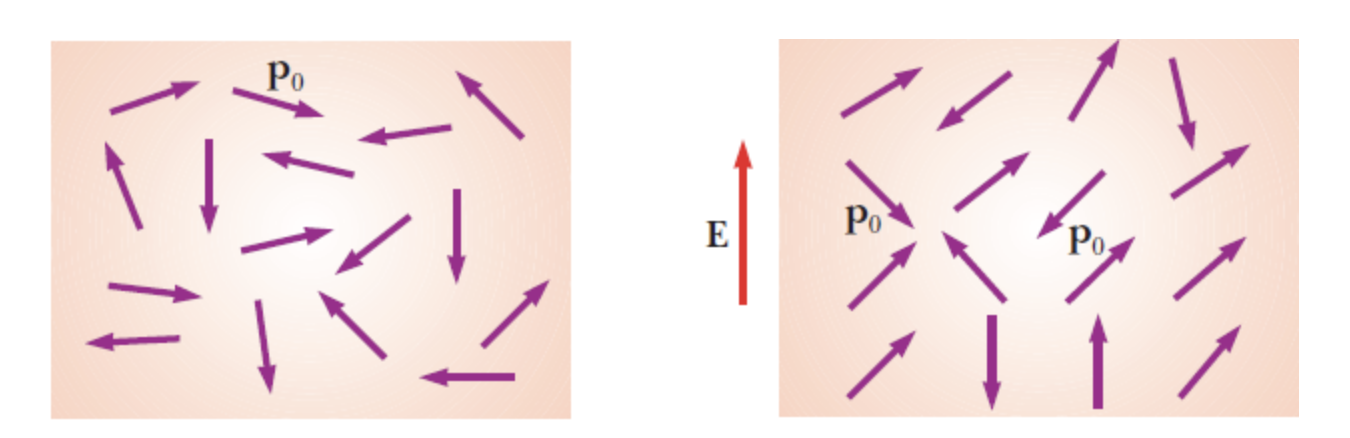
\includegraphics[width=0.8\linewidth]{figure/image23.png}
    \caption{Azione del campo elettrostatico sulle molecole di una sostanza dotate di momento di dipolo intrinseco}
    \label{fig:chapter_11_1}
\end{figure}

Allora possiamo andare ad ipotizzare che ciascuna molecola acquisti un \emph{momento di dipolo medio} $< \mathbf{p} >$ microscopico \emph{parallelo} al campo elettrostatico $\mathbf{E}$. \\

Considerato un volumetto $\Delta \tau$ del dielettrico, contenente $\Delta N$ atomi (o molecole), il momento di dipolo risultante è dato dal prodotto $\Delta N  <\mathbf{p}>$ e il momento di dipolo elettrico per unità di volume è dato da 

\begin{equation}
    \mathbf{P} = \frac{\Delta N}{\Delta \tau} < \mathbf{p} >
\end{equation}

Il \mkeyword{polarizzazione del dielettrico} vettore $\mathbf{P}$ che caratterizza l'effetto di formazione dei momenti di dipolo indotti dal campo esterno, si chiama \emph{polarizzazione del dielettrico}.\\
In particolare se facciamo tendere $\Delta \tau$ a zero, otteniamo il valore di $\mathbf{P}$ in uno specifico punto del dielettrico. \\

\newpage

Esiste un'importante tipologia di dielettrici che prende \mkeyword{dielettrici lineari} il nome di dielettrici \emph{lineari}.\\ 
Un dielettrico lineare è un materiale in cui la \emph{polarizzazione $\mathbf{P}$ è proporzionale al campo elettrico applicato $\mathbf{E}$}, in particolare:

\begin{tcolorbox}[colback=yellow!10!white, colframe=orange!70!black, boxrule=0.8pt]
\begin{equation}
    \mathbf{P} = \varepsilon_0 (\kappa_e - 1) \mathbf{E} = \varepsilon_0 \chi_e \mathbf{E}
\end{equation}
\end{tcolorbox}

Dove $\kappa_e$ prende il \mkeyword{costante dielettrica relativa del dielettrico} nome di \emph{costante dielettrica relativa del dielettrico}, mentre $\chi_e$ prende il nome di \mkeyword{suscettività elettrica del dielettrico}  \emph{suscettività elettrica del dielettrico}.\\
Queste due grandezze \emph{dipendono solamente dalla natura del dielettrico, indipendentemente dalla geometria e grandezza}.\\

Per il resto del capitolo \emph{andiamo a ipotizzare che i dielettrici considerati siano lineari}.\\

\' E possibile fare un'ulteriore suddivisione tra i dielettrici: \emph{isotropi} e \emph{anisotropi}. \\

Un dielettrico è isotropo quando la sua polarizzazione in ogni punto è parallela al campo elettrico $\mathbf{E}$, cioè quando $\chi_e$ è uno scalare. \\

\' E anisotropo quando la sua polarizzazione non è parallela al campo e $\chi_e$ è un 2-tensore (una matrice 3x3). \\

\section{Campo elettrico prodotto da un dielettrico polarizzato}

Supponiamo di avere un dielettrico soggetto a un campo elettrico, per quanto visto sopra il momento di dipolo di ciascuna molecola sarà modificato, questo comporta che \emph{il dielettrico stesso genera un campo elettrico}.\\

Andiamo a trovare il campo elettrico generato dal dielettrico. Per semplicità di calcolo ricaviamo il potenziale (cosa che ci porta a conoscere anche il campo).\\

Possiamo andare a suddividere il dielettrico in un numero infinito di parti, ciascuna delle quali rappresenta un dipolo.\\ Per ogni parte vale

\begin{equation*}
    V(\mathbf{r}) = \frac{1}{4 \pi \varepsilon_0} \frac{\mathbf{p} \cdot \mathbf{u}_r}{r^2}
\end{equation*}

dove $\mathbf{r}$ è il vettore che va dal dipolo al punto nello spazio dove vogliamo trovare il potenziale. \\

Per come abbiamo definito $\mathbf{P}$, possiamo affermare che $\mathbf{p} = \mathbf{P} d\tau'$ in tutti gli infinitesimi volumi $d \tau '$ in cui abbiamo diviso il materiale.\footnote{con " ' " si va a indicare che quella grandezza si riferisce al particolare punto del dielettrico} \\

Allora tutto il potenziale in un punto risulta essere 

\begin{equation}
    V(\mathbf{r}) = \frac{1}{4 \pi \varepsilon_0} \int_{\tau} \frac{\mathbf{P}(\mathbf{r'}) \cdot \mathbf{u}_r}{r^2} \ d \tau '
\end{equation}

In principio questo basterebbe, ma possiamo fare un'importante osservazione 

\begin{equation}
    \nabla \left(\frac{1}{r} \right) = \frac{\mathbf{u}_r}{r^2}
\end{equation}

Quindi

\begin{equation*}
    V = \frac{1}{4 \pi \varepsilon_0} \int_{\tau} \mathbf{P} \cdot \nabla \left(\frac{1}{r} \right) \ d\tau '
\end{equation*}

Sappiamo che vale 

\begin{equation*}
    \mathbf{P} \cdot \nabla \left(\frac{1}{r} \right) = \nabla \cdot \left(\frac{\mathbf{P}}{r} \right) - \frac{1}{r} \ (\nabla \cdot \mathbf{P})
\end{equation*}

Allora sostituendo

\begin{equation*}
     V = \frac{1}{4 \pi \varepsilon_0} \left [ \int_{\tau}  \nabla \cdot \left(\frac{\mathbf{P}}{r} \right) \ d\tau ' - \int_{\tau} \frac{1}{r} (\nabla \cdot \mathbf{P}) \ d \tau '\right ]
\end{equation*}

Applicando il teorema della divergenza 

\begin{tcolorbox}[colback=yellow!10!white, colframe=orange!70!black, boxrule=0.8pt]
\begin{equation}
         V = \frac{1}{4 \pi \varepsilon_0}  \oint_{\Sigma}  \frac{\mathbf{1}}{r} \ \mathbf{P} \cdot \mathbf{\hat{n}} \ d\Sigma ' - \frac{1}{4 \pi \varepsilon_0} \int_{\tau} \frac{1}{r} (\nabla \cdot \mathbf{P}) \ d \tau '
\end{equation}
\end{tcolorbox}

Si nota che il primo termine sembra molto il potenziale di una superficie di carica 

\begin{tcolorbox}[colback=yellow!10!white, colframe=orange!70!black, boxrule=0.8pt]
\begin{equation}
    \sigma_p \equiv \mathbf{P} \cdot \mathbf{\hat{n}}
\end{equation}
\end{tcolorbox}

Dove $\sigma_p$ è la \mkeyword{densità superficiale delle cariche polarizzate} \emph{densità superficiale delle cariche polarizzate}, mentre $\mathbf{\hat{n}}$ è il versore tangente alla superficie del dielettrico e \emph{uscente} da questa. \\

Mentre il secondo termine assomiglia a un potenziale di volume di carica 

\begin{tcolorbox}[colback=yellow!10!white, colframe=orange!70!black, boxrule=0.8pt]
\begin{equation}
    \rho_p \equiv - \nabla \cdot \mathbf{P}
\end{equation}
\end{tcolorbox}

Dove \mkeyword{densità volumica delle cariche polarizzate} $\rho_p$ è la \emph{densità volumica delle cariche polarizzate}.\\

\newpage

\subsection{Interpretazione fisica delle cariche di polarizzazione}

Queste cariche potrebbero sembrare "fittizie" - semplici strumenti per facilitare il calcolo dei campi. Tuttavia non è così, $\rho_p $ e $ \sigma_p$ rappresentano accumuli di carica perfettamente autentici. \\

L'idea di base è molto semplice: supponiamo che la polarizzazione $\mathbf{P}$ sia uniforme, e supponiamo di avere una lunga serie di dipoli.

\begin{figure}[h]
    \centering
    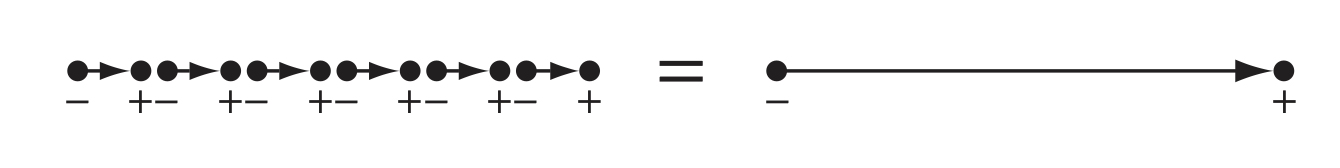
\includegraphics[width=0.65\linewidth]{figure/image24.png}
    \caption{Linea di dipoli}
    \label{fig:chapter_11_2}
\end{figure}

La testa di uno annulla di fatto la coda del
suo vicino, ma alle estremità rimangono due cariche: $+$ all'estremità destra e $-$ a quella sinistra. È come se avessimo staccato un elettrone da un'estremità e lo avessimo portato
fino all'altra estremità, anche se in realtà nessun singolo elettrone ha percorso
l'intero percorso: molti piccoli spostamenti si sommano per formare un unico grande spostamento.\\

Se la polarizzazione è non uniforme, otteniamo un accumulo di cariche anche all'\emph{interno} del materiale oltre che sulla superficie (le cariche dei dipoli il linea non si annullano sovrapponendosi).

\section{Equazioni dell'elettrostatica in presenza di dielettrici}

Dal momento che il campo prodotto da cariche elettriche è conservativo anche in presenza di dielettrici polarizzati, continuano a valere le due condizioni, integrale e locale, date da

\begin{equation*}
    \oint \mathbf{E} \cdot d \mathbf{s} = 0 \quad , \quad  \nabla \times \mathbf{E} = 0
\end{equation*}

e la proprietà equivalente che il campo elettrostatico si possa ottenere come gradiente della funzione potenziale, $\mathbf{E} = - \nabla V$. \\

Anche la legge di Gauss resta valida in presenza di dielettrici polarizzati, \emph{purché si tenga conto delle cariche di polarizzazione oltre che delle cariche libere}:

\begin{tcolorbox}[colback=yellow!10!white, colframe=orange!70!black, boxrule=0.8pt]
\begin{equation}
    \oint_{\Sigma} \mathbf{E} \cdot \mathbf{u}_n \ d \Sigma = \frac{q + q_p}{\varepsilon_0}
\end{equation}
\end{tcolorbox}

Deduciamo la forma locale 

\begin{tcolorbox}[colback=yellow!10!white, colframe=orange!70!black, boxrule=0.8pt]
\begin{equation}
    \nabla \cdot \mathbf{E} = \frac{\rho + \rho_p}{\varepsilon_0}
\end{equation}
\end{tcolorbox}

\newpage

Allora, si nota facilmente che 

\begin{equation}
    \varepsilon_0 \nabla \cdot \mathbf{E} = \nabla \cdot \varepsilon_0 \mathbf{E} = \rho - \nabla \cdot \mathbf{P} \implies \nabla \cdot (\varepsilon_0 \mathbf{E} + \mathbf{P}) = \rho
\end{equation}

a cui corrisponde l'integrale 

\begin{equation}
    \oint_{\Sigma} (\varepsilon_0 \mathbf{E} + \mathbf{P}) \cdot \mathbf{u}_n \ d \Sigma = q
\end{equation}

Allora possiamo andare a definire una nuova grandezza vettoriale 

\begin{tcolorbox}[colback=yellow!10!white, colframe=orange!70!black, boxrule=0.8pt]
\begin{equation}
    \mathbf{D} = \varepsilon_0 \mathbf{E} + \mathbf{P}
\end{equation}
\end{tcolorbox}

Dove $\mathbf{D}$ prende \mkeyword{induzione dielettrica} il nome di \emph{induzione dielettrica}. \\

Allora possiamo scrivere:

\begin{tcolorbox}[colback=yellow!10!white, colframe=orange!70!black, boxrule=0.8pt]
\begin{equation}
    \nabla \cdot \mathbf{D} = \rho \quad , \quad \oint_{\Sigma} \mathbf{D} \cdot \mathbf{u}_n \ d \Sigma = q
\end{equation}
\end{tcolorbox}

Il flusso del vettore induzione dielettrica $\mathbf{D}$ attraverso una superficie chiusa, contenente in generale sia cariche libere che cariche polarizzate, \emph{dipende soltanto dalle cariche libere}. \\

Per completezza aggiungiamo che per il vettore induzione dielettrica non si può stabilire che la circuitazione lungo qualsiasi percorso chiuso è nulla: $\mathbf{D}$ non è cioè un campo conservativo. \\

\subsection{Relazioni per dielettrici lineari}

Dato che stiamo trattando dielettrici lineari, è possibile travare una relazione diretta tra $\mathbf{D}$ e $\mathbf{E}$ e tra $\mathbf{D}$ e $\mathbf{P}$. Sostituendo

\begin{equation*}
    \mathbf{P} = \varepsilon_0 (\kappa_e - 1) \mathbf{E} = \varepsilon_0 \chi_e \mathbf{E}
\end{equation*}

nella definizione di induzione elettrica si ottengono le seguenti relazioni:

\begin{tcolorbox}[colback=yellow!10!white, colframe=orange!70!black, boxrule=0.8pt]
\begin{equation}
    \mathbf{D} = \varepsilon_0 \kappa_e \mathbf{E} = \varepsilon \mathbf{E}
    \label{eq:legame_D_E}
\end{equation}
\end{tcolorbox}

Dove \mkeyword{costante dielettrica assoluta} $\varepsilon$ è definito come il prodotto tra $\varepsilon_0$ e $\kappa_e$ e prende il nome di costante dielettrica assoluta del dielettrico. 

\begin{tcolorbox}[colback=yellow!10!white, colframe=orange!70!black, boxrule=0.8pt]
\begin{equation}
    \mathbf{P} = \frac{\kappa_e - 1}{\kappa_e} \mathbf{D} = \frac{\chi_e}{1 + \chi_e} \mathbf{D}
\end{equation}
\end{tcolorbox}

\newpage

In particolare si ottiene che $\nabla \cdot \mathbf{P} \propto \nabla \cdot \mathbf{D}$, quindi se $\nabla \cdot \mathbf{D} = 0$ vale che 

\begin{equation}
    \rho_p = - \nabla \cdot \mathbf{P} = 0  
\end{equation}

Cioè in un dielettrico lineare e omogeneo la densità spaziale di carica di polarizzazione è nulla e le cariche di polarizzazione sono distribuite esclusivamente sulle superfici.  

\section{Discontinuità dei campi sulla superficie di separazione tra due dielettrici}

Andiamo a vedere come si comporta un campo elettrostatico quando attraversa una superficie di separazione tra due dielettrici con costante dielettrica diversa. \\

Supponiamo di avere due dielettrici con costante dielettrica relativa $\kappa_{e_1}$ e $\kappa_{e_2}$ e sia $\Sigma$ la superficie di separazione. Indichiamo con $\mathbf{E}_1$, $\mathbf{P}_1$ , $\mathbf{D}_1$ rispettivamente il campo elettrostatico, la polarizzazione e l'induzione dielettrica sulla faccia di $\Sigma$ rivolta al dielettrico di costante dielettrica $\kappa_{e_1}$  e con $\mathbf{E}_2$, $\mathbf{P}_2$ , $\mathbf{D}_2$ i corrispettivi valori sulla faccia di $\Sigma$ rivolta al secondo dielettrico. \\

\begin{figure}[h]
    \centering
    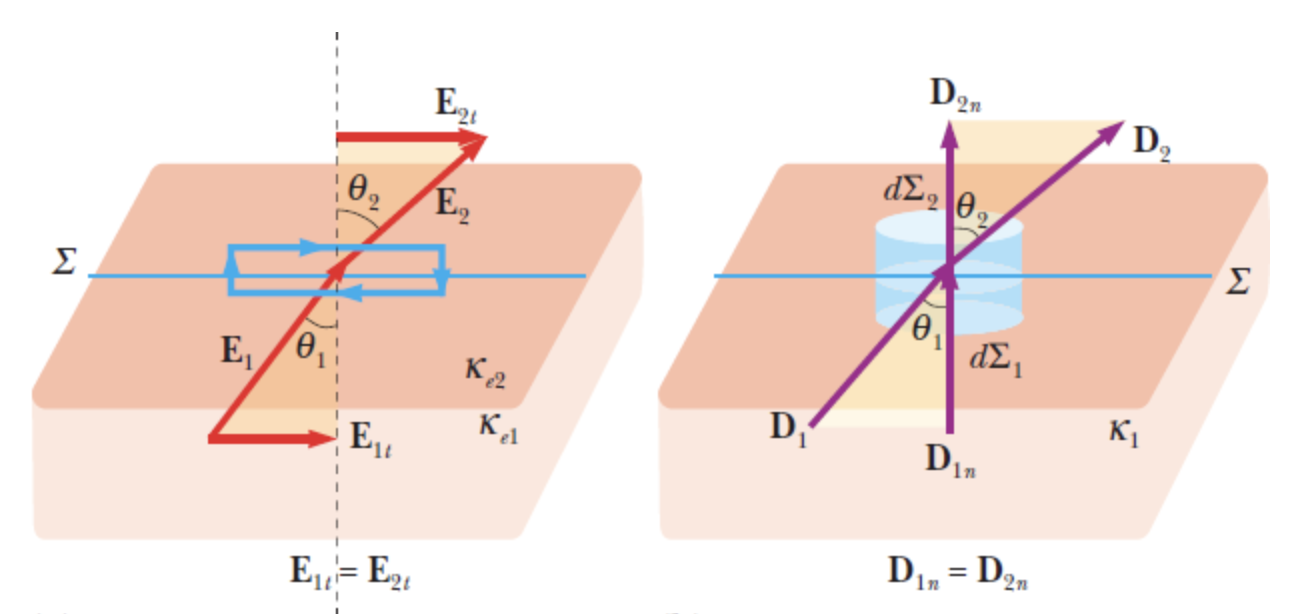
\includegraphics[width=0.7\linewidth]{figure/image25.png}
    \caption{}
    \label{fig:dielettrici_mezzi}
\end{figure}

Vediamo cosa succede alla componente tangenziale al piano del campo elettrico nel passaggio attraverso $\Sigma$.\\

Consideriamo una linea chiusa rettangolare che attraversa $\Sigma$ e in cui la lunghezza dei lati perpendicolari alla superficie è molto minore della lunghezza dei lati paralleli (come in Figura \ref{fig:dielettrici_mezzi}). Essendo entrambi i campi elettrici conservati, deve valere

\begin{equation}
    \oint \mathbf{E} \cdot d \mathbf{s} = 0 \implies E_{1t} \ l - E_{1t} \ l = 0
\end{equation}

Nella relazione abbiamo approssimati i lati perpendicolari. Allora otteniamo 

\begin{tcolorbox}[colback=yellow!10!white, colframe=orange!70!black, boxrule=0.8pt]
\begin{equation}
    E_{1t} = E_1 \sin \theta_1 = E_2 \sin \theta_2 = E_{2t}
\end{equation}
\end{tcolorbox}

Cioè la componente tangenziale di $\mathbf{E}$ rimane costante nel passaggio attraverso $\Sigma$. \\


Applichiamo adesso la legge di Gauss al vettore $\mathbf{D}$, scegliendo per superficie chiusa di integrazione una scatola cilindrica di altezza infinitesima ortogonale a $\Sigma$ e con le basi $d \Sigma_1$ di normali $\mathbf{u}_{n_1}$ e $d \Sigma_2$ di normale $\mathbf{u}_{n_2}$ all'interno dei due dielettrici. 

\begin{equation}
    \oint_{\Sigma'} \mathbf{D} \cdot \mathbf{u}_n ' \ d \Sigma ' = \mathbf{D}_2 \cdot \mathbf{u}_{n_2} \ d \Sigma + \mathbf{D}_1 \cdot \mathbf{u}_{n_1} \ d \Sigma = (D_{2n} - D_{1n}) d\Sigma = 0 
\end{equation}

Ma allora vale che 

\begin{tcolorbox}[colback=yellow!10!white, colframe=orange!70!black, boxrule=0.8pt]
\begin{equation}
    D_{1n} = D_{2n}
\end{equation}
\end{tcolorbox}

Inoltre dalla relazione \ref{eq:legame_D_E} otteniamo:

\begin{tcolorbox}[colback=yellow!10!white, colframe=orange!70!black, boxrule=0.8pt]
\begin{equation}
    \kappa_{e_1} \varepsilon_0 E_1 \cos \theta_1 = \kappa_{e_2} \varepsilon_0 E_2 \cos \theta_2
\end{equation}
\end{tcolorbox}

E dividendo membro a membro 

\begin{tcolorbox}[colback=yellow!10!white, colframe=orange!70!black, boxrule=0.8pt]
\begin{equation}
    \frac{\text{tg} \theta_1}{\text{tg} \theta_2} = \frac{\kappa_{e_1}}{\kappa_{e_2}}
\end{equation}
\end{tcolorbox}

La discontinuità della componente normale di $\mathbf{E}$, insieme alla continuità della componente tangenziale, comporta un cambiamento di direzione delle linee di forza del campo elettrostatico. 

\newpage

\subsection{Problemi al contorno con i dielettrici}
I metodi usati nei capitoli precedenti per la soluzione di problemi di valori al contorno possono essere facilmente applicati anche in presenza di dielettrici. In questo paragrafo tratteremo alcuni esempi delle varie tecniche applicate a mezzi dielettrici. 

\subsubsection{Carica entro un dielettrico semi-infinito}

Consideriamo una carica puntiforme $q$ disposta entro un dielettrico semi-infinito di costante dielettrica \emph{assoluta} $\varepsilon_1$ ad una distanza $d$ dal piano di separazione del primo mezzo da un secondo dielettrico dielettrico semi-infinito di costante $\varepsilon_2$. Il piano di separazione sia il piano $z = 0$. 

\begin{figure}[h]
    \centering
    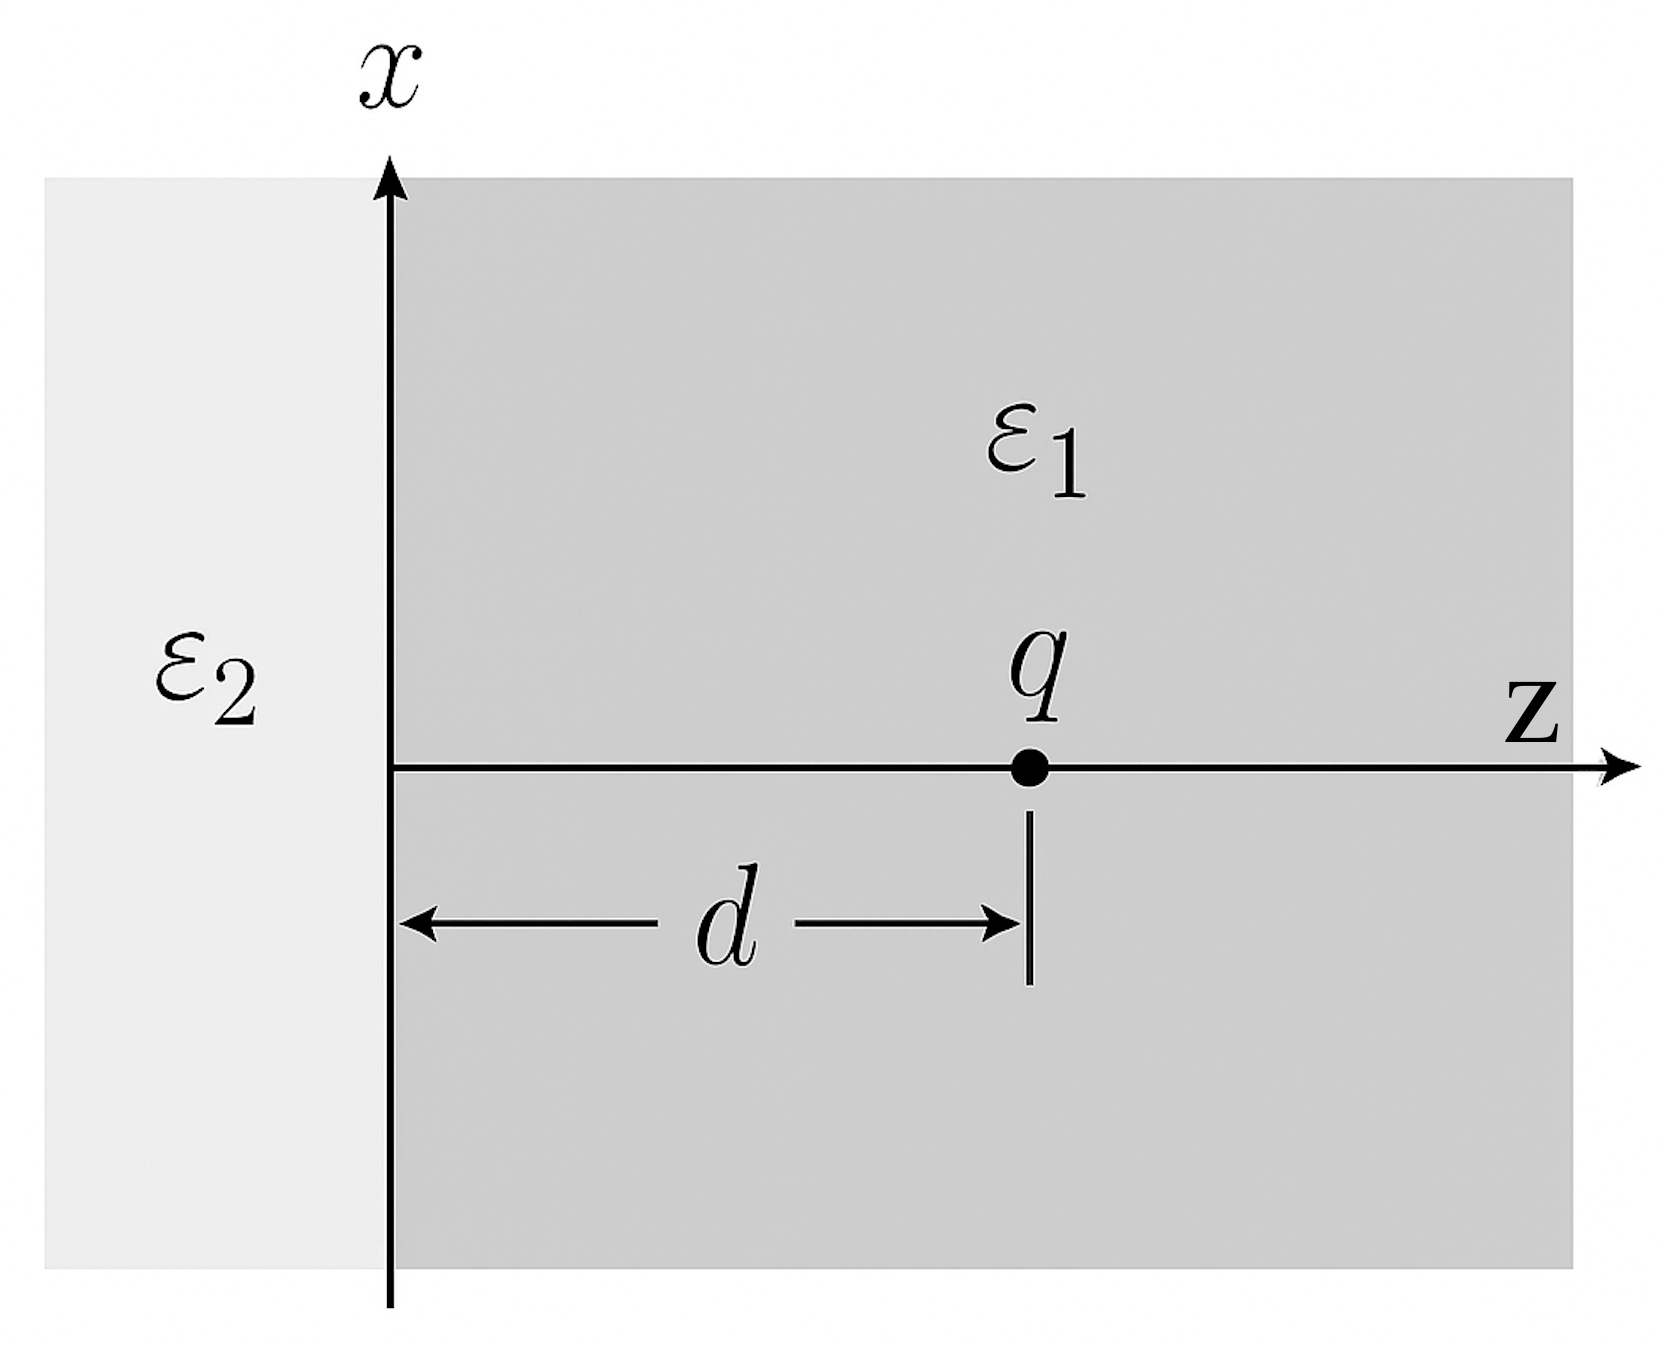
\includegraphics[width=0.35\linewidth]{figure/image26.png}
    \caption{Dielettrici semi-infiniti}
    \label{fig:chapter_11_3}
\end{figure}

Dobbiamo trovare una soluzione appropriata per le condizioni

\begin{align*}
    \varepsilon_1 \nabla \cdot E = \rho \quad  \quad z >0\\
    \varepsilon_2 \nabla \cdot E = 0 \quad  \quad z <0
\end{align*}

Le condizioni al contorno per $z = 0$ sono :

\begin{equation}
    \lim_{z \to 0^{+}} \colvec{ \varepsilon_1 E_z \\ E_x \\ E_y} = \lim_{z \to 0^{-}} \colvec{ \varepsilon_2 E_z \\ E_x \\ E_y}
    \label{eq:condizioni_dipoli}
\end{equation}

Volendo usare il metodo delle cariche immagine per trovare il potenziale nel semispazio contenente la carica, appare naturale disporre una carica immagine $q'$ posta nella posizione simmetrica $A'$ rispetto alla posizione $A$ della carica $q$. 

\begin{figure}[h]
    \centering
    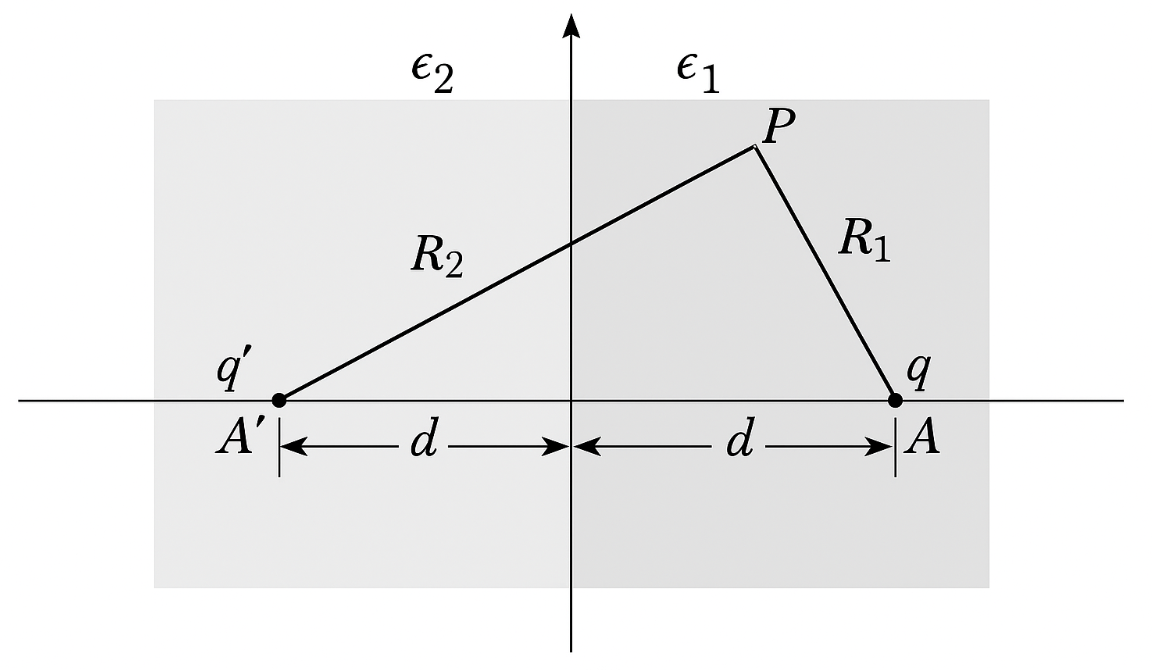
\includegraphics[width=0.55\linewidth]{figure/image27.png}
    \caption{}
    \label{fig:chapter_11_4}
\end{figure}

\newpage

Allora per $z > 0$ il potenziale nel punto $P$ di coordinate cilindriche $(\rho, \theta,z)$ sarà 

\begin{equation}
    V(\rho, \theta, z) = \frac{1}{4 \pi \varepsilon_1} \left( \frac{q}{R_1} + \frac{q'}{R_2} \right) \qquad z >0
\end{equation}

dove $R_1 = \sqrt{\rho^2 + (d-z)^2}$ e $R_2 = \sqrt{\rho^2 + (d + z)^2}$. \\

Ora dobbiamo trovare il potenziale per $z<0$. Siccome in questo semispazio non ci sono cariche, il potenziale deve essere soluzione della equazione di Laplace senza singolarità. L'ipotesi più semplice è evidentemente che per $z<0$ il potenziale sia equivalente a quello di una carica $q''$ nella posizione $A$ della carica effettiva q:

\begin{equation}
    V(\rho, \theta, z) = \frac{1}{4 \pi \varepsilon_2} \frac{q''}{R_1} \qquad z<0
\end{equation}

Dato che 

\begin{equation*}
    \frac{\partial}{\partial z} \left ( \frac{1}{R_1} \right)_{z = 0} = -\frac{\partial}{\partial z} \left ( \frac{1}{R_2} \right)_{z = 0} = \frac{d}{(\rho^2 + d^2)^{3/2}}
\end{equation*}

Mentre

\begin{equation*}
    \frac{\partial}{\partial \rho} \left ( \frac{1}{R_1} \right)_{z = 0} = \frac{\partial}{\partial \rho} \left ( \frac{1}{R_2} \right)_{z = 0} = - \frac{\rho}{(\rho^2 + d^2)^{3/2}}
\end{equation*}

Allora dalle condizioni al bordo \ref{eq:condizioni_dipoli} otteniamo

\begin{equation}
    \begin{cases}
        q-q' = q''\\
        \frac{1}{\varepsilon_1} (q + q') = \frac{1}{\varepsilon_2} q''
    \end{cases}
\end{equation}

Risolvendo il sistema si ottiene che 

\begin{tcolorbox}[colback=yellow!10!white, colframe=orange!70!black, boxrule=0.8pt]
\begin{equation}
    q' = -\left( \frac{\varepsilon_2 - \varepsilon_1}{\varepsilon_2 + \varepsilon_1} \right) q \quad ,  \quad q'' = \left( \frac{2 \varepsilon_2}{\varepsilon_2 + \varepsilon_1} \right)
\end{equation}
\end{tcolorbox}

\subsubsection{Sfera dielettrica in campo uniforme}

Consideriamo una sfera di dielettrico di raggio $a$ con costante dielettrica relativa $\varepsilon/\varepsilon_0$, soggetta a un campo elettrostatico uniforme.

\begin{figure} [h]
    \centering
    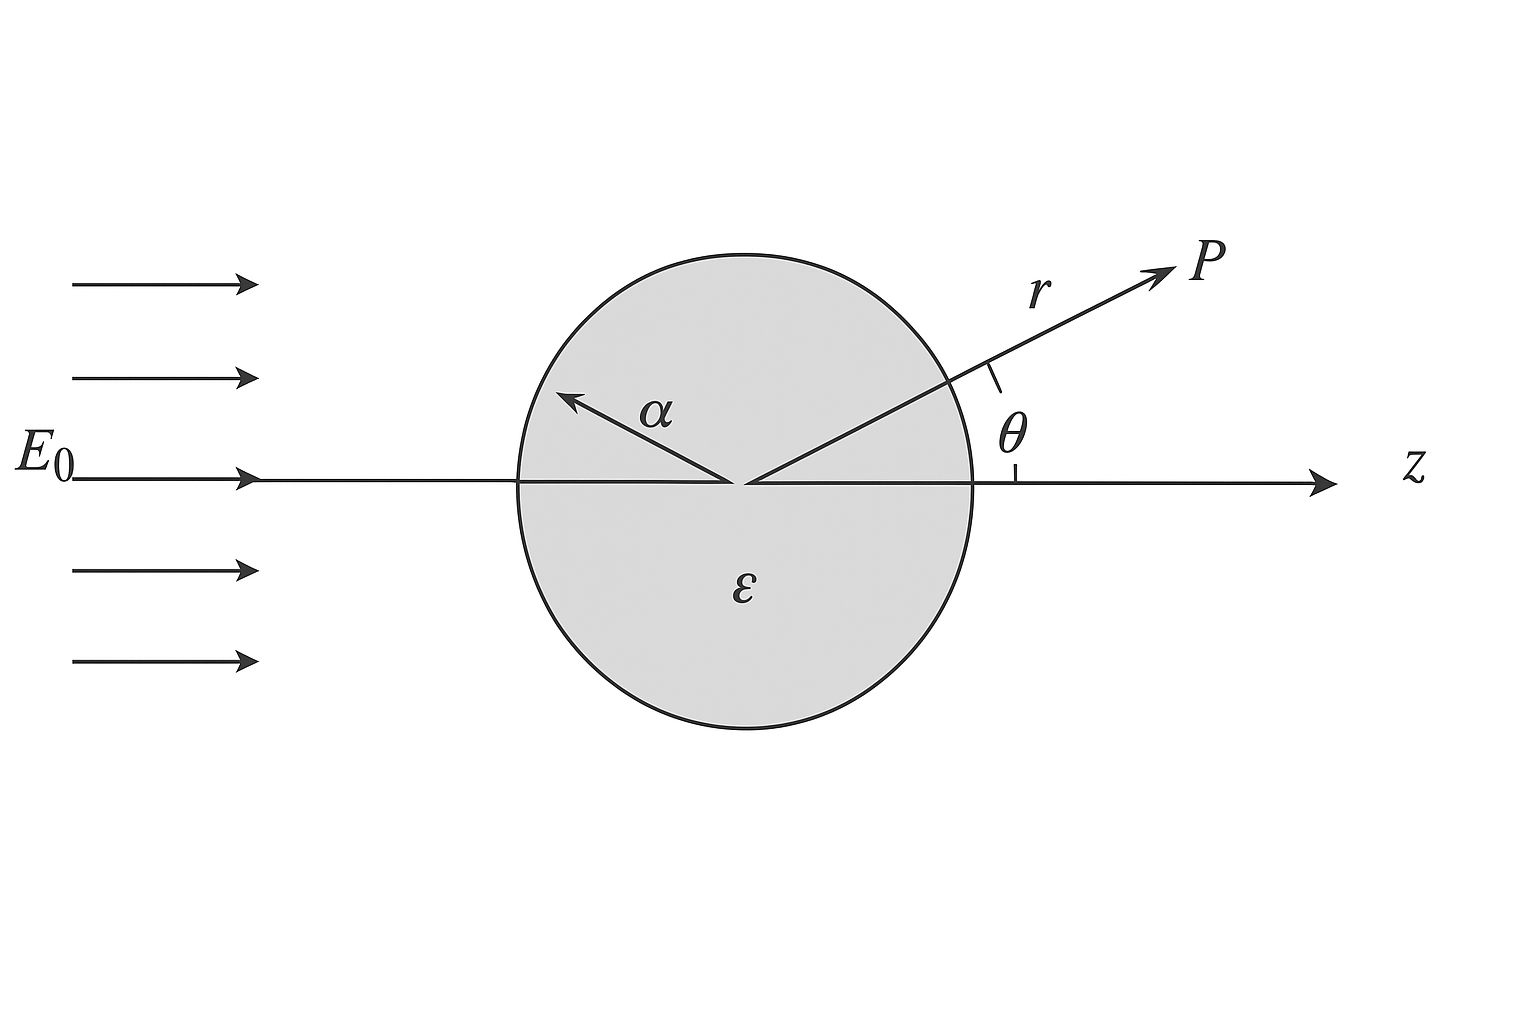
\includegraphics[width=0.5\linewidth]{figure/image28.png}
    \caption{Sfera di dielettrico in campo uniforme}
    \label{fig:chapter_11_5}
\end{figure}

Applicando il metodo di separazione delle variabili e sfruttando la simmetria azimutale del sistema, possiamo sapere la forma del potenziale all'interno e all'esterno della sfera:

\begin{equation}
    V_{in} (r, \theta) = \sum_{l= 0}^{+ \infty} A_l r^l P_l (\cos \theta) \qquad , \qquad V_{est}(r, \theta) = \sum_{l = 0} ^ {+ \infty} \left ( B_l r^l + C_l \frac{1}{r^{l+1}} \right) P_l (\cos \theta)
\end{equation}

Si sottolinea il fatto che nel potenziale all'interno della sfera i coefficienti dei termini $1/r^{l+1}$ sono nulla in quanto all'interno della sfera è contenuta anche l'origine del sistema. \\

Andiamo ad imporre le condizioni al contorno per trovare il valore dei coefficienti. \\

Dalla condizione all'infinito ($V \to - E_0 z = - E_0 \cos \theta$) si trova che l'unico coefficiente $B_l$ che non si annulla è $B_1 = -E_0$.\\

Gli altri coefficienti si trovano grazie alle condizioni al contorno per $r = a$:\\

La condizione tangenziale alla superficie

\begin{align*}
    - \frac{1}{a} \frac{\partial V_{in}}{\partial \theta} _{r= a} = - \frac{1}{a} \frac{\partial V_{est}}{\partial \theta} _{r= a}\\
\end{align*}

La condizione normale alla superficie

\begin{equation*}
    -\varepsilon \frac{\partial V_{in}}{\partial r} _{r = a} =  -\varepsilon \frac{\partial V_{est}}{\partial r} _{r = a} \quad
\end{equation*}

Una volta fatta la sostituzione si ottengono due serie di funzioni di Legendre uguali a zero. Dato che si devono annullare per qualsiasi $\theta$, i coefficienti di ciascuna funzione di Legendre deve annullarsi separatamente. Si ottengono le seguenti condizioni:

\begin{equation}
    \begin{cases}
        A_1 = - E_0 + \frac{C_1}{a^3} \\
        A_l = \frac{C_l}{a^{2l +1}} \quad  l\neq 1\\
        (\varepsilon/\varepsilon_0) A_1 = - E_0 - 2 \frac{C_1}{a^3}\\
        (\varepsilon/\varepsilon_0) l A_l = - (l+1) \frac{C_l}{a^{2l +1}} \quad l\neq 1
    \end{cases}
\end{equation}

Le condizioni riguardanti le $l$ possono essere soddisfatte contemporaneamente se e solo se $A_l = C_l = 0$ per $l \neq 1$. Allora risulta

\begin{align}
    A_l = - \left ( \frac{3}{2 + \varepsilon/\varepsilon_0} \right) E_0\\
    C_l = \left( \frac{\varepsilon/\varepsilon_0 - 1}{\varepsilon/\varepsilon_0 + 2} \right) a^3 E_0
\end{align}

\newpage

Allora i potenziali diventano 

\begin{tcolorbox}[colback=yellow!10!white, colframe=orange!70!black, boxrule=0.8pt]
\begin{align}
    V_{in} (r, \theta) = - \left ( \frac{3}{2 + \varepsilon/\varepsilon_0} \right) E_0 \ r \cos \theta\\
    V_{est} (r, \theta) = - E_0 r \cos \theta + \left( \frac{\varepsilon/\varepsilon_0 - 1}{\varepsilon/\varepsilon_0 + 2} \right) E_0 \frac{a^3}{r^2} \cos \theta
\end{align}
\end{tcolorbox}

Si nota allora che al di fuori della sfera sfera il potenziale è equivalente al potenziale dovuto al campo uniforme $E_0$ e al campo di un dipolo posto nell'origine con momenti di dipolo:

\begin{tcolorbox}[colback=yellow!10!white, colframe=orange!70!black, boxrule=0.8pt]
\begin{equation}
    p = 4 \pi \varepsilon_0 \left( \frac{\varepsilon/\varepsilon_0 - 1}{\varepsilon/\varepsilon_0 + 2} \right) a^3 E_0
\end{equation}
\end{tcolorbox}

Questo momento di dipolo può essere interpretato come l'integrale di volume della polarizzazione $\mathbf{P}$, quindi risulta 

\begin{tcolorbox}[colback=yellow!10!white, colframe=orange!70!black, boxrule=0.8pt]
\begin{equation}
    \mathbf{P} = 3 \varepsilon_0 \left( \frac{\varepsilon/\varepsilon_0 - 1}{\varepsilon/\varepsilon_0 + 2} \right)  \mathbf{E}_0
\end{equation}
\end{tcolorbox}

\section{Energia elettrostatica nei dielettrici}

Consideriamo un sistema formato da un dielettrico e da delle cariche libere e vogliamo trovare l'energia elettrostatica di tale sistema. \\

Supponiamo di considerare il dielettrico fisso nello spazio e di aggiungere una alla volta le cariche libere. Con l'aumentare la densità delle cariche libere $\rho$ di una quantità $\Delta \rho$, cambierà anche la densità di polarizzazione del dielettrico; tuttavia, noi siamo interessati solo nel lavoro svolto per aumentare le cariche \emph{libere}:

\begin{equation}
    \Delta W  = \int (\Delta \rho) V \ d \tau
\end{equation}

Dato che $\nabla \cdot \mathbf{D} = \rho $, $\Delta \rho = \nabla \cdot (\Delta \mathbf{D})$, quindi 

\begin{equation*}
    \Delta W = \int [\nabla \cdot (\Delta \mathbf{D})] V \ d \tau
\end{equation*}


Sappiamo 

\begin{equation*}
    \nabla \cdot [(\Delta \mathbf{D} \ V)] = [\nabla \cdot (\Delta \mathbf{D})] V + \Delta \mathbf{D} \cdot (\nabla V)
\end{equation*}

Allora otteniamo 

\begin{equation*}
    \Delta W = \int \nabla \cdot [(\Delta \mathbf{D)} V ] \ d \tau + \int (\Delta \mathbf{D}) \cdot \mathbf{E} \ d \tau
\end{equation*}

Applicando il teorema della divergenza, si trasforma il primo integrale in un integrale di superficie, che scompare se integriamo in tutto lo spazio. \\

Allora 

\begin{equation*}
    \Delta W = \int (\Delta \mathbf{D}) \cdot \mathbf{E} \ d \tau
\end{equation*}

Fino a questo punto il ragionamento è applicabile a qualsiasi dielettrico. Ora, se andiamo a ipotizzare che il dielettrico sia lineare (come abbiamo fatto fino ad ora), vale $\mathbf{D} = \varepsilon \mathbf{E}$, quindi 

\begin{equation*}
    (\Delta \mathbf{D}) \cdot \mathbf{E} = \varepsilon(\Delta \mathbf{E}) \cdot \mathbf{E} = \frac{1}{2} \Delta (\varepsilon E^2) = \frac{1}{2} \Delta (\mathbf{D} \cdot \mathbf{E})
\end{equation*}

Allora 

\begin{equation*}
    \Delta W = \Delta \left( \frac{1}{2} \int \mathbf{D} \cdot \mathbf{E} \ d \tau\right)
\end{equation*}

Il lavoro totale fatto per raggiungere il sistema desiderato da zero è proprio l'energia del sistema, quindi risulta 

\begin{tcolorbox}[colback=yellow!10!white, colframe=orange!70!black, boxrule=0.8pt]
\begin{equation}
    U_e = \frac{1}{2} \int \mathbf{D} \cdot \mathbf{E} \ d \tau
\end{equation}
\end{tcolorbox}
